\documentclass[letterpaper,preprint]{aastex62}
\usepackage{bm}
\usepackage{calc}
\usepackage{amssymb, amsmath}
\usepackage{hyperref}
\newcounter{address}
\newcommand{\doctype}{paper}
\newcommand{\equationname}{equation}
\newcommand{\eqnref}[1]{\mbox{\equationname~\ref{#1}}}
\newcommand{\appref}[1]{\mbox{Appendix~\ref{#1}}}
\newcommand{\Appref}[1]{\mbox{Appendix~\ref{#1}}}
\newcommand{\tabref}[1]{\mbox{Table~\ref{#1}}}

\newcommand{\niceurl}[1]{\mbox{\href{#1}{\textsl{#1}}}}

\newcommand{\latin}[1]{\emph{#1}}
\newcommand{\etal}{\latin{et\,al.}}
\newcommand{\ie}{\latin{i.e.}}
\newcommand{\apriori}{\latin{a priori}}
\newcommand{\sn}{{[s/n]}}
\newcommand{\sntotal}{\sn_{\mathrm{total}}}
\newcommand{\fwhm}{{\theta_{\mathrm{FWHM}}}}
\newcommand{\RA}{{\mathrm{RA}}}
\newcommand{\Dec}{{\mathrm{Dec}}}
\newcommand{\vecmu}{\bm{\vec{\mu}}}
\newcommand{\mualpha}{{\mu_\alpha}}
\newcommand{\mudelta}{{\mu_\delta}}
\newcommand{\var}[1]{\mathrm{Var}({#1})}
\newcommand{\unit}[1]{\mathrm{#1}}
\renewcommand{\mag}{\unit{mag}}
\newcommand{\s}{\unit{s}}
\newcommand{\yr}{\unit{yr}}
\newcommand{\km}{\unit{km}}
\newcommand{\pc}{\unit{pc}}
\newcommand{\kpc}{\unit{kpc}}
\newcommand{\mas}{\unit{mas}}
\newcommand{\pix}{\unit{pix}}
\newcommand{\kmpers}{\km\,\s^{-1}}
\newcommand{\masperyr}{\mas\,\yr^{-1}}
\renewcommand{\arcsec}{\unit{arcsec}}
\newcommand{\arcsecperyr}{\arcsec\,\yr^{-1}}
\newcommand{\code}[1]{\texttt{#1}}
\newcommand{\mean}[1]{\left<{#1}\right>}

\renewcommand{\thefootnote}{\fnsymbol{footnote}}

\newcommand{\figpart}[1]{\textbf{#1}}
%\newcommand{\fig}{Figure}
%\newcommand{\figref}[1]{\mbox{\fig~\ref{#1}}}
\newcommand{\figref}[1]{\mbox{Figure~\ref{#1}}}
\newcommand{\detmap}{detection map}
\newcommand{\Detmap}{Detection map}
\newcommand{\fluxmap}{flux map}
\newcommand{\fmap}{F}
\newcommand{\drawnfrom}{\sim}
\newcommand{\gaussianN}{\mathcal{N}}
\newcommand{\gaussian}[1]{\gaussianN\!\left(#1\right)}
%\newcommand{\gaussx}[2]{\hat{\gaussianN}\!\left(#1 \, , \, #2\right)}
\newcommand{\gaussx}[2]{\gaussianN\!\left(#1 \, , \, #2\right)}
%\newcommand{\gaussx}[1]{\mathfrak{N}\!\left(#1\right)}
%\newcommand{\psf}{\mathrm{psf}}
\newcommand{\psf}{\psi}
\newcommand{\psfat}[1]{\psf_{#1}}
\newcommand{\psfnorm}{\norm{\bm{\psf}}}

\newcommand{\signoise}{[S/N]}
\newcommand{\snr}[1]{\mathbb{SN}(#1)}
%\newcommand{\snr}[1]{\mathcal{SN}(#1)}

\newcommand{\norm}[1]{\left\lVert #1 \right\rVert}
\newcommand{\expect}[1]{\left\langle #1 \right\rangle}
\renewcommand{\var}[1]{\mathrm{var}\left( #1 \right)}
\newcommand{\sky}{\mathrm{sky}}
\newcommand{\psfw}{w}
\newcommand{\dd}{\mathrm{d}}
\newcommand{\noise}{e}
\renewcommand{\vec}[1]{\boldsymbol{#1}}
\newcommand{\thetavec}{\vec{\theta}}
\newcommand{\avec}{\vec{a}}
\newcommand{\ivec}{\vec{i}}
\newcommand{\jvec}{\vec{j}}
\newcommand{\kvec}{\vec{k}}
\newcommand{\cvec}{\vec{c}}
\newcommand{\posvec}{\vec{x}}
\newcommand{\coord}[2]{(#1, #2)}
\newcommand{\iina}{\ivec \,\, \mathrm{in} \,\, \mathcal{A}}

\begin{document}
\title{Principled point-source detection in collections of astronomical images}
\author{Dustin Lang}
%\altaffiliation{To whom correspondence should be addressed; \texttt{dstndstn@gmail.com}}
\affiliation{%
  Dunlap Institute and Department for Astronomy \& Astrophysics,
  University of Toronto,
  50 Saint George Street, Toronto, ON, M5S 3H4, Canada}
\affiliation{%
  Visitor, Department of Physics \& Astronomy,
  University of Waterloo,
  200 University Avenue West, Waterloo, ON, N2L 3G1, Canada}
\affiliation{%
  Visitor, Perimeter Institute for Theoretical Physics,
  31 Caroline Street North, Waterloo, ON, N2L 2Y5, Canada}

\author{David W. Hogg}
\affiliation{%
  Center for Cosmology and Particle Physics,
  Department of Physics,
  New York University, 4 Washington Place, New York, NY 10003, USA}
\affiliation{%
  Max-Planck-Institut f\"ur Astronomie,
  K\"onigstuhl 17, D-69117 Heidelberg, Germany}

\correspondingauthor{Dustin Lang}
\email{dstndstn@gmail.com}

\begin{abstract}
We review the well-known \emph{matched filter} method for the
detection of point sources in astronomical images.  This is shown to
be optimal (that is, to saturate the Cram\'er--Rao bound) under stated
conditions that are very strong: an isolated source in
background-dominated imaging with perfectly known background level,
point-spread function, and noise models.  We show that the matched
filter produces a maximum-likelihood estimate of the brightness of a
purported point source, and this leads to a simple way to combine
multiple images---taken through the same bandpass filter but with
different background levels and point-spread functions---to produce an
optimal point source detection map.  We then extend the approach to
images taken through different bandpass filters, introducing the
\emph{SED-matched filter}, which allows us to combine images taken
through different filters, but requires us to specify the colors of
the objects we wish to detect.  We show that this approach is superior
to some methods traditionally employed, such as the \emph{chi-squared
  coadd} (Szalay \emph{et al.} 1999), and that other traditional
methods can be seen as instances of SED-matched filtering with implied
(and often unreasonable) priors.
%
% We suggest a set of SED filters and how one ought to proceed: lower
% the detection threshold to ensure that all sources of interest are
% detected, then fit for their properties and keep or discard sources
% based on their utility for the question at hand.
%
\end{abstract}

\keywords{
    methods:~statistical ---
    techniques:~image~processing
}

FIXME -- are we going to talk about detecting galaxies?  Seems like we
should!

FIXME -- should we talk about the probability of selecting the wrong
pixel as the peak?

FIXME -- need some consistent way of labelling image quantities, and
sensible naming and careful use of ``flux'' and ``counts''.  Some
notation for ``estimates for'' or ``maximum-likelihood point estimate
of'' would be useful too.  Hats?


\section{Introduction}

There are few operations in astronomy more important than the
detection of stars or point sources.
Indeed, many astronomical discoveries come down to point-source
detection.
What is the best method for performing such detection?
Here we answer that question, in the limited context of isolated
sources, uniform sky-limited noise, and well-understood point-spread
function.
Even in this limited context, the subject is rich and valuable; more
general---and more difficult---cases will be illuminated if we can
understand the simplest case first.

Fundamentally, when much is understood about a signal latent in noisy
data, the best detection methods are (or look like) \emph{matched
filters}.
A matched filter is a model of the expected signal with which the data
are \emph{cross-correlated}. % (often wrongly called ``convolved'').
Peaks in the cross-correlation are candidate signal detections.
In point-source detection in astronomical images, the expected signal is the
point-spread function (PSF), and the cross-correlation operation is often
wrongly called ``convolution by the PSF''.
Matched filters are well used in astronomy, in contexts ranging from
spectroscopy (CITE) to
galaxy clusters \cite{redmapper, melin} to
ultra-faint galaxies \cite{willman1} to
exoplanets \cite{exoplanet} to
gravitational radiation \cite{ligo}.

% from the tweeps:
% http://scholar.google.com/scholar?q=astronomy+matched+filter
% http://arxiv.org/abs/astro-ph/0602424

In what follows, we will argue for matched filtering for point-source
detection.  This is not new (CITE); what is new is that we consider
the common context of heterogeneous (in point-spread function and
sensitivity) multi-epoch, multi-band imaging.
%
While the optimality of matched filtering for single-image point
source detection is well known by astronomers, the straightforward
mathematics behind it is often not, leading to a misconception that
it is simply an algorithmic choice.  To our knowledge, the optimal%
\footnote{In this \doctype\ we use ``optimal'' in a technical sense,
 of saturating the Cram\'er--Rao bound under stated assumptions.  We
 encourage other authors to do the same!}
method of combining multiple images with different properties to
obtain the greatest possible sensitivity to point sources has not been
written down in the astronomical literature.  The mathematics are
straightforward and the resulting procedure is simple and
computationally inexpensive.  

Perhaps more controversially, we go on to argue that when imaging in
multiple bands is available, one should again use a matched filter,
now matched to the spectral-energy distribution (SED) of the sources
to be detected.  This SED-matched filtering, as we will call it, makes
explicit the assumptions that are implicitly embedded in any method
that attempts to detect sources by combining imaging from multiple
bands.

In the Real World, astronomers never precisely know their point-spread
function, their noise model, their flat-field (or other calibration
parameters), nor the spectral-energy distributions of the sources of
greatest interest.
Also, often, the sources of interest aren't point sources or perhaps
vary with time.
In these cases, we advocate parameterizing ignorance, and operating
with the union of all possibly appropriate matched filters.
We will fully execute this idea here when it comes to spectral-energy
distributions, but there are natural extensions to deal with
point-spread function, noise-model, calibration, and time-domain
uncertainties.

% FIXME -- DISCUSS each of the things listed above in the Discussion (or omit)!



A ``traditional'' approach for detecting sources in multi-epoch
imaging is to co-add the images and then run a detection algorithm on
the resulting coadd.  When the images have different point-spread
functions or noise properties, this method results in needless loss of
sensitivity; producing a coadd effectively forces the use of a
\emph{mismatched filter} rather than a matched filter.  We will show
that the correct procedure involves creating a weighted co-addition of
matched-filtered (smoothed) images.

% Often, astronomers ``co-add'' their imaging to find faint
% objects.  Technically, this step is only justifiable if the bandpass
% and point-spread function are the same for all images, and the images
% ought to be weighted somehow according to sensitivity.  Co-addition is
% not necessary for source detection, of course; it is possible to
% combine low-significance source-detection information coming from many
% images and do as well or better than co-addition.  

% An amusing
% conclusion of this project is that in the principled limit, the
% combination of source-detection information looks very much like a
% (weighted) co-addition of (smoothed) data!

That is, in what follows, we will detect sources as above-threshold
pixels or regions in a weighted co-add of PSF-correlated input images.
We will call this object a ``detection map''.  This detection map is
the best thing to use for source detection.  Once sources are
detected, of course, the detection map should be put aside, and source
properties (positions, colors, and so on) ought to be measured
(inferred) from the raw pixels in the collection of input images via a
likelihood function.  That measurement and likelihood function is
beyond the scope of this paper, but the subject of a parallel research
program (eg, \cite{unwise-phot}).

\section{Our image model}

We consider idealized astronomical images such as those obtained from
a CCD in typical broadband optical imaging.
Specifically, we will make the following strong assumptions:
\begin{itemize}
\item the noise (coming from such sources as the Poisson distribution
  of the sky background, dark current, and read noise) is zero-mean,
  Gaussian, pixelwise independent, and of known constant variance.  The
  zero-mean assumption can be seen as assuming perfect background
  subtraction (sky estimation);
\item the image is well sampled;
\item the (perhaps tiny) image contains \emph{only} one point
  source with some (unknown) flux and position;
\item the source is centered within a pixel (we will relax this
  later);
\item the point-spread function is spatially constant (across the
  possibly small image patch of interest) and known perfectly;
\item the device is linear and the photometric calibration of the
  image is known perfectly; that is, that it is possible to map from
  ``count'' units back to physical units or a photometric standard;
\item the image is perfectly astrometrically calibrated;
\item the image is not contaminated by cosmic rays, stray light, bad
  pixels, bad columns, electronic artifacts, or any other of the many
  defects in real images.
\end{itemize}

Throughout this \doctype\ we assume a ``pixel-correlated'' PSF; we
consider the point-spread function to \emph{include} the effects of
pixelization.  In well-sampled images, we think of the image as being
a continuous function which, after being correlated by the PSF, is
sampled at delta-function pixel locations.  There is no need to think
of pixels as ``little boxes''; they are simply samples of an
underlying smooth two-dimensional signal.

% FIXME -- mention that the pixel-sampled PSF is the thing we actually
% have access to in the images. (ie, if we use known stars to construct
% a PSF model)


With these strong assumptions, we can write down the probability
distribution of each pixel value, which allows us to prove the
optimality of the methods we present.
%
We will consider a discrete image made up of a square array of pixels
$\jvec$, each of which has value $I_{\jvec}$, where we
use $\jvec$ as a two-dimensional focal-plane position, measured in
integer pixel units.
%
If the image contains a single point source, centered on
the pixel at position $\kvec$ and with constant flux resulting in a
total number of counts $F$, then the image is
\begin{eqnarray}
  I_{\jvec} &=& F \, \psfat{\jvec - \kvec} + \noise_{\jvec} \quad ,
  \label{eqn:image}
\end{eqnarray}
where $\psi(\jvec-\kvec)$ is the point-spread function evaluated at
offset $\jvec-\kvec$ and $\noise_{\jvec}$ is per-pixel noise drawn
from a zero-mean Gaussian with known, constant, per-pixel variance $\sigma_1^2$.
%
We can also write this as
\begin{eqnarray}
  I_{\jvec} &\drawnfrom& \gaussx{F \, \psfat{\jvec - \kvec}}{\sigma_1^2}
  \quad ,
\end{eqnarray}
meaning that $I_{\jvec}$ is drawn from a Gaussian distribution with
mean $F\, \psf(\jvec - \kvec)$ and variance $\sigma_1^2$.


\section{Detecting a point source in a single image}

%\subsection{Optimal linear detection}

Here we consider a point source $k$ in a single image, as in
\eqnref{eqn:image}.

% the map $M_{\jvec}$ can
% be computed by correlating the image with its PSF:
% \begin{equation}
% M_{\jvec} = \sum_{\iina} \psi_{\ivec} \, S_{\ivec + \jvec} \quad ,
% \end{equation}
% where, as before, $\mathcal{A}$ is the support of the PSF and
% $\psfat{\ivec} = \psi(\ivec)$ is an image of the PSF evaluated at
% integer pixel positions $\ivec$.

The \emph{matched filtering} operation, also known as ``smoothing by
the PSF'' or ``correlating by the PSF''\footnote{
  Or, often, ``convolving by the PSF'', being slightly careless with terminology.}
can be written as
\begin{eqnarray}
  M_{\jvec} &=& \sum_{\iina} \psfat{\ivec} \, I_{\ivec + \jvec} \quad ,
\end{eqnarray}
where $\mathcal{A}$ is the support of the PSF and $\psfat{\ivec} =
\psf(\ivec)$ is an image of the PSF evaluated at integer pixel
positions $\ivec$.  This operation can be seen as ``gathering up'' the
signal that is dispersed into many pixels by the PSF, weighting by the
fraction of the flux that went into the pixel.  In
\appref{app:lindet} we derive the matched filter and show that it
saturates the Cram\'er--Rao bound.

% In \appref{app:lindet}\ we show that \emph{correlating} an image by
% its PSF---\emph{matched filtering}---results in an optimal detector
% for isolated point sources.  This operation can be seen as ``gathering
% up'' the signal that is dispersed into many pixels by the PSF; or as
% re-scaling each pixel in the support of the PSF into an estimate of
% the total flux and producing a weighted average of these estimates.

We define the \emph{\detmap} $D_{\jvec}$ as the matched filter, scaled to be in convenient units:
\begin{equation}
D_{\jvec} = \frac{1}{\psfnorm^2} \sum_{\iina} \psfat{\ivec} \,
I_{\ivec + \jvec} \quad ,
\label{eq:detmap}
\end{equation}
%where $\mathcal{A}$ is the support of the PSF and
%$\psfat{\ivec} = \psf(\ivec)$ is an image of the PSF model evaluated at
%integer-offset pixel positions $\ivec$.
The PSF norm $\psfnorm$ is
\begin{equation}
\psfnorm = \sqrt{\sum_{\iina} \psfat{\ivec}^2} \quad ,
\end{equation}
and as shown in \appref{app:gaussnorm}, a Gaussian PSF with standard
devation $\psfw$ pixels has a norm approximately:
\begin{equation}
  \norm{\bm{\psf^G}} \simeq \frac{1}{2 \sqrt{\pi} \psfw} \quad .
\end{equation}
The per-pixel error in the \detmap\ is given by
\begin{equation}
\sigma_{D} = \frac{\sigma_1}{\psfnorm} \quad .
\end{equation}


We have scaled the \detmap\ so that each pixel contains the
maximum-likelihood estimate of the total counts of a source centered
at that pixel.  That is, if we compute at pixel $\jvec$ the total
source counts $F^{\ast}_{\jvec}$ to minimizes the chi-squared
($\chi^2$) residual within the support of the PSF:
\begin{equation}
  F^{\ast}_{\jvec} = \arg\min_{f} \sum_{\ivec} \left( \frac{I_{\ivec+\jvec} - f \, \psfat{\ivec}}{\sigma_1} \right)^2
\end{equation}
we find
\begin{eqnarray}
  F^{\ast}_{\jvec} &=& \frac{\sum_{\ivec} I_{\ivec+\jvec} \, \psfat{\ivec}}{\sum_{\ivec} \psfat{\ivec}^2}
  \\
  F^{\ast}_{\jvec} &=& D_{\jvec} %\quad .
\end{eqnarray}
as defined above.
%
That is, a significant peak in the \detmap\ indicates the likely
position of a point source, and the value of the \detmap\ at a pixel
is the maximum-likelihood estimate of the total source counts for a
source centered at that pixel.


\subsection{Threshold and Peaks}

% In astronomical imaging, and in particular in large-scale surveys, it

Once we have computed a detection map, we typically wish to produce a
list of detected sources.  Standard practice is to apply a threshold
at, say, $5 \sigma_D$, and accept any peak above that threshold as a
source (or a blended group of sources).\footnote{%
  ``Deblending'' nearby groups of sources is a challenging task that
  is beyond the scope of this paper.}
In regions containing no
sources, the detection map contains Gaussian noise.  Due to the
correlation operation, the detection map pixels are not pixelwise
independent, but as weighted sums of Gaussian samples they remain
Gaussian.  As such, the expected number of pixels above a threshold
$\tau$ is the integral of the high tail of the normal distribution.
For $\tau = 5 \sigma_D$, the fraction of pixels above threshold due to
noise is about $2.9\times10^{-7}$, which seems tiny except that we
will be evaluating millions of pixels; in a 4k$\times$4k image we
would expect approximately $5$ false positive detections.

There is nothing special about $5 \sigma$ as a detection threshold; it
is simply a choice of tradeoff between allowing some false positives
while preventing too many false negatives (lost detections).  In
different situations, higher or lower thresholds could be preferable.

\subsection{Comments}

\paragraph{PSF model}
Computing the detection map requires correlation of the image by a
model of its point-spread function.  In practice, the PSF model is
never known exactly, and since correlation by large pixelized models
can be expensive, it is common to approximate the PSF by a Gaussian
for the purposes of detecting sources.  The impact this approximation
of the PSF has on detection efficiency is apparent in the derivation
of the matched filter; in equation \ref{eqn:psfdotprod}, the detection
map signal-to-noise is proportional to the cosine distance between the
true PSF and the correlation kernel.  In typical ground-based images,
this results in only a few percent loss in signal-to-noise.  For
example, in our Legacy Surveys images, if we assume that our pixelized
model of the PSF is correct, then a Gaussian approximation typically
yields above $97\%$ efficiency.

\paragraph{Biases}
In this paper, we have assumed that backgrounds due to atmospheric
emission (``sky'') and detector effects such as bias and dark current
have been perfectly estimated and subtracted.  In real images,
however, errors in these estimates can leave spatially coherent
residual biases, and these can have a considerable effect on source
detection.  For example, a background that is elevated by $0.05
\sigma_1$ per pixel can double the $5\sigma$ false positive rate in
good seeing, and has an even greater effect in worse seeing.

% Specifically, sky bias on detection:
% D_j / sigma_D = 1/||psf||^2 (\sum_i \psf_i (C_i + b)) / (sigma_1/||psf||)
%               = 1/(||psf|| sigma_1) (\sum_i \psf_i C_i + b)
% if b = \beta \sigma_1, D_j / sigma_D is offset by
%  \beta / ||psf||

% ||psf_G(width = 1)|| ~ 0.282
% so a sky bias of 0.05 sigma per pixel yields a shift of 0.177 sigma;
%
%scipy.special.erfc((5. - 0.05/0.282)/np.sqrt(2.))/2.
%-> 7.081571486838887e-07
% Which is over twice the 5-sigma FP rate.

% Peak statistics in Gaussian fields
% Rice 1944, 1945
% Longuet-Higgins 1957 (2-d)

% scipy.special.erf = 2/sqrt(pi)*integral(exp(-t**2), t=0..z)

% vs normal 1/sqrt(2 pi sigma^2) exp(-(x-mu)^2/(2 sigma^2))

% Fraction in high tail of N(1,0) above tau:
% f = (1.-scipy.special.erf(tau / np.sqrt(2.))) / 2
% f = scipy.special.erfc(tau /np.sqrt(2.))/2.

% 5 sigma:
% scipy.special.erfc(5./np.sqrt(2.))/2.
% 2.866515718791945e-07

% 4.9 sigma: scipy.special.erfc(4.9/np.sqrt(2.))/2.
% 4.791832765903203e-07

% 4.5 sigma: scipy.special.erfc(4.5/np.sqrt(2.))/2.
% 3.3976731247300607e-06



% \paragraph{Convolution.}  It is common to hear the statement
% that \emph{convolving} an image by its PSF model yields an optimal
% detection filter.  This is only true if the PSF is defined to be
% ``flipped'' in both axes relative to the image coordinate system.  We
% prefer to define the PSF in unflipped coordinates, so correlation
% rather than convolution is the correct operation (they are equivalent
% when the PSF model is symmetric).

% \paragraph{Multiple sources.}
% We emphasize that we focus on detecting \emph{isolated point sources}
% in this \doctype.  In particular, we are ignoring important
% practicalities such as blended sources


% -- Sub-pixel peak location...

\paragraph{Sub-pixel peaks}  The detection map defined above
is computed by correlating the image with its PSF, on the image pixel
grid.  As the PSF becomes narrow, the detection efficiency varies
depending on the position of a source within the pixel.  The detection
map is maximized when the image is a scaled version of the PSF
(matched filter), but if the image is shifted within a pixel relative
to the PSF model, then the peak value attained by the detection map is
lower (because the filter is slightly mismatched).  For example, with
a Gaussian PSF with standard deviation of 1 pixel, the detection map
drops as low as 88\% efficiency for a source midway between pixels in
both dimensions.

To reduce this effect, one could compute multiple detection maps,
using for each a different subpixel-shifted versions of the PSF model.
Alternatively, one could lower the detection threshold to compensate,
then fit for the best source position and drop sources with best-fit
values below threshold.


\paragraph{Sufficient statistic}  Correlation by the PSF summarizes
all relevant information regarding the presence of a source at each
pixel; the detection map and its variance are sufficient to describe
our knowledge.  In some astronomical source detection packages
(including SourceExtractor), there is a notion of requiring more than
one neighboring pixel to exceed a detection threshold.  This is not
necessary or useful; in effect it imposes a larger detection threshold
that varies based on the source morphology and PSF, which is
undesirable.


% \paragraph{What would Bayes do?}  FIXME -- We haven't really explained that
% we are producing and evaluating an estimate for each pixel.  Could
% also point out that one could instantiate and test the generative
% model (with position and flux) at each pixel, and that this basically
% just short-cuts that process, telling you places where that test is
% going to give significant results.

\paragraph{Galaxies}
We have focused only on point sources, but the same arguments can be
used to develop a detector for galaxies.  The matched filter by which
the image must be correlated is then the intrinsic galaxy profile
correlated with the PSF; a matched-filtering approach is only optimal
for a given galaxy profile.  As with using an approximation for the
PSF model, the non-optimality due to using an incorrect galaxy profile
is related to the cosine distance between the correct and model galaxy
profile.

In practice, our mixture-of-Gaussians approximations to standard
exponential and deVaucouleurs galaxy profiles \cite{gaussgals} are
convenient for this task.



\section{Detecting a point source in multiple images}

In this section we will assume we have a stationary point source whose
flux is constant over time, and a series of images taken through
different bandpass filters and with different noise levels, exposure
times, point-spread functions, and telescope pointings.  We can
achieve optimal detection of the source by building a \detmap\ for
each image and combining them with weights as described below.



\subsection{Identical bandpass filters}

We first present the simpler case where all the images are taken
through identical bandpass filters.

As we have seen, the \detmap\ defined in \eqnref{eq:detmap} is a
maximum-likelihood estimate of the total \emph{counts} contributed by
the source, in the units of the original image.  In order to
combine information from multiple images, we must calibrate them so
that they are in the same units.  Since this calibration is simply a
linear scaling, it can be applied to the original image or to the
\detmap.  Similarly, if the images are on different pixel
grids---either from different pointings of the same CCD, or from
different CCDs---then we must \emph{resample} the \detmap s to a
common pixel grid.
%
If the original image is well-sampled, then the \detmap\ (which has
been further smoothed by PSF correlation) will also be well-sampled,
so resampling to a pixel grid of the same or finer resolution results
in no loss of information.
%
Since the pixel values in the \detmap\ represent the \emph{total} flux
from a point source, the \detmap\ does not need to be rescaled when
resampled to a different pixel scale.



Once the \detmap\ for each image has been calibrated and resampled to
a common pixel grid, we have multiple \emph{independent}
maximum-likelihood estimates of the source flux in our chosen filter,
each with a known standard deviation and Gaussian statistics.  That
is, we have multiple Gaussian likelihood functions that we wish to
combine.  Since they are independent, the combined likelihood is the
product of the individual likelihoods.  For Gaussian distributions,
the resulting aggregate maximum likelihood estimate is the
inverse-variance-weighted sum of the individual estimates.

If the calibration factor $\kappa_i$ scales image $i$ to flux in
common units, and $R_i$ represents resampling to the common pixel grid,
then the flux estimate $F_i$ is
\begin{eqnarray}
F_i &=& R_i(\kappa_i \, D_i)
\end{eqnarray}
with per-pixel error
\begin{eqnarray}
\sigma_{F, i} &=& \frac{\kappa_i \, \sigma_{1,i}}{\psfnorm_i}
\end{eqnarray}
and we combine the estimates from multiple images via
\begin{eqnarray}
F^{\star} &=& \frac{\displaystyle\sum_i F_i \, \sigma^{-2}_{F,i}}{\displaystyle\sum_i \sigma^{-2}_{F_i}}
\label{eq:onebandmap}
\end{eqnarray}
which has per-pixel error
\begin{eqnarray}
  \sigma_{F, \star} &=& \left( \sum_i \sigma^{-2}_{F,i} \right)^{-\frac{1}{2}}    \quad .
  \label{eq:onebandstd}
\end{eqnarray}
This is simply the maximum-likelihood estimate of the flux based on a
set of independent Gaussian estimates.


In summary, the procedure to produce an optimal detection map given
multiple images (in the same filter) is:
\begin{enumerate}
\item \emph{correlate} each image by its PSF model
\item \emph{calibrate} each resulting detection map (and its variance)
  to common units
\item \emph{resample} each calibrated detection map to a common pixel
  grid
\item \emph{coadd} the calibrated detection maps weighted by their
  inverse variances.
\end{enumerate}
Assuming well-sampled images, the \emph{correlation},
\emph{calibration}, and \emph{resampling} steps can occur in any
order.  Importantly, however, the \emph{coaddition} stage must occur
\emph{after} correlation by the point-spread functions of the
individual images; each image must be correlated by its own matched
filter to produce \emph{detection maps} which are then coadded.

\subsection{Comments}

\paragraph{Optimality}
In appendix \ref{app:multiopt} we show that the estimator $F^{\star}$
saturates the Cram\'er--Rao bound and is therefore statistically
optimal.

\paragraph{Coadds}
Occasionally, astronomers attempt to construct image coadds and then
detect sources by correlating the coadd with an estimate of its PSF.
It is straightforward to show that this is necessarily sub-optimal
unless the images have the same PSF.  Intuitively, the PSF of the
coadd is not equal to the PSF of either image, therefore this approach
uses a ``mismatched filter'' rather than a matched filter, resulting
in loss of signal-to-noise or detection efficiency.

\begin{figure}[h]
  \begin{center}
  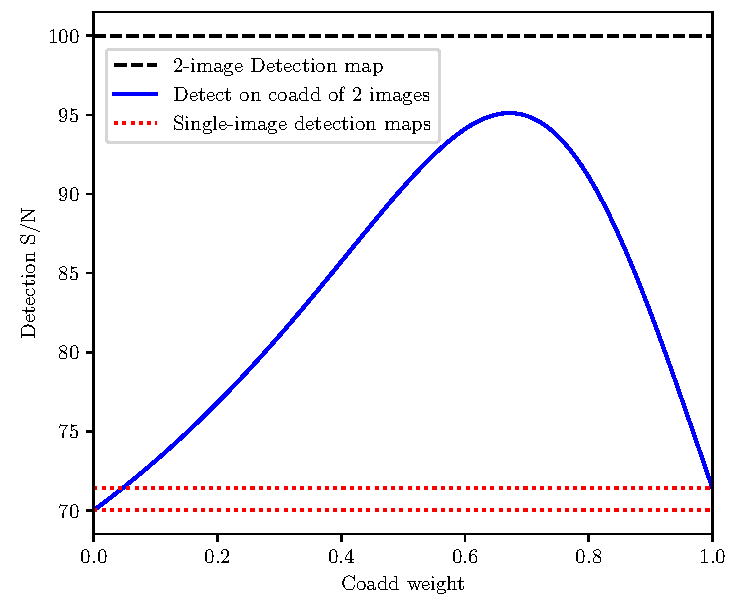
\includegraphics[width=0.5\textwidth]{dont-coadd}
  \caption{Loss of signal-to-noise in computing a coadd and detecting
    sources in the codad, rather than computing the detection map on
    the individual images.  Two images, with PSF widths differing by a
    factor of two, and exposure times such that the depths are
    similar, are coadded and sources detected.  Regardless of the
    weighting used to coadd the images, detection efficiency is lost
    compared to the method presented in this paper.\label{fig:dontcoadd}}
  \end{center}
\end{figure}

%
As an illustration, we simulated two images with similar detection
signal-to-noise but Gaussian PSFs that differed by a factor of two.
We computed the detection map, and also created a series of coadds
(trying different weights for the two images), computing the detection
map for each, using the correct coadded PSF.  As shown in Figure
\ref{fig:dontcoadd}, regardless of the coadd weight chosen, detecting
on the coadd results in a loss of efficiency compared to the detection
map.


\subsection{Different bandpass filters}

As we saw in the single-bandpass case, we can combine multiple
individual exposures into an aggregate estimate of the flux of a point
source.  In order to do this, it was essential to calibrate the images
so that each one was an estimate of the same underlying quantity.  The
multiple-bandpass case is similar: For each bandpass, we first combine
the images taken in that bandpass into an aggregate estimate.  Then,
to combine the bandpasses we must scale them so that they are
estimates of the same quantity.  This requires \emph{knowing} the
spectral energy distribution, or at least the \emph{colors} in the
filters of interest, of the source to be detected; this allows us to
scale the various bandpasses so that they are estimates of a common
quantity: perhaps the flux in a canonical band, or some other linear
quantity such as the integrated intensity.

%% FIXME -- does that make sense?  Apparent brightness?  Apparent
%% luminosity?  I just want to say, you could measure it in anything
%% linear, like W/m^2/sr/s or, heck, the projected area of a star of a
%% given temperature)


The intuition here is that if we know that our sources of interest are
twice as bright in bandpass A as in bandpass B, then we can convert
an estimate of the brightness in band B into an estimate of the
brightness in band A by multiplying by two.  The variance of the
scaled estimate increases appropriately (by a factor of four), so a
bandpass in which a source is expected to be faint will contribute an
estimate with a large variance and will be downweighted when the
estimates are combined.  We can also view the problem as one of
estimating a total flux that has been split into the different
bandpasses, and in that view it is analogous to the way flux is spread
into pixels by the point-spread function.

\newcommand{\sigdj}{\sigma_{j}}

Assume we have computed detection maps $D_j$, with per-pixel standard deviation
$\sigdj$, for a number of different bandpasses.  Assume each
bandpass has a known conversion factor $f_j$ to the canonical band;
that is,
\begin{eqnarray}
  D_j & \drawnfrom & \gaussx{f_j F}{\sigdj^2}
\end{eqnarray}
for flux in the canonical band $F$.
% \footnote{% The notation $x
%   \drawnfrom \gaussx{\mu}{\sigma^2}$ means that $x$ is drawn from a
%   Gaussian distribution with mean $\mu$ and variance $\sigma^2$.}
%
Given a number of such detection maps, we first scale them so they are all estimates of the
same quantity, by dividing by $f_j$:
\begin{eqnarray}
  F_j & = & \frac{D_j}{f_j} \\
  F_j & \drawnfrom & \gaussx{F}{\frac{\sigdj^2}{f_j^2}}
\end{eqnarray}
and assuming that the images  are independent, we combine them by inverse-variance weighting
to produce the maximum-likelihood estimate for $F$:
\begin{eqnarray}
  \hat{F} &=& 
  %\frac{\sum_j D_j \, f_j \, \sigdj^{-2}}%
  %     {\sum_j f_j^2 \, \sigdj^{-2}}
  \frac{\displaystyle\sum_j \frac{D_j}{f_j} \, \frac{f_j^2}{\sigdj^2}}%
       {\displaystyle\sum_j \frac{f_j^2}{\sigdj^2}}
       = 
       \frac{\displaystyle\sum_j D_j \, f_j \, \sigdj^{-2}}%
            {\displaystyle\sum_j f_j^2 \, \sigdj^{-2}}
\end{eqnarray}
with per-pixel error
\begin{eqnarray}
  \hat{\sigma}_F &=& \left( \sum_j f_j^2 \sigdj^{-2} \right)^{-\frac{1}{2}}
  \quad .
\end{eqnarray}


For example, if we treat $r$ band as the canonical band and our
objects of interest have color $r-i = 1$, then we 
expect the flux in $i$ to be a factor of $2.5$ greater than the
flux in $r$; $f_i = 2.5$, and we
will scale our
$i$-band detection map $D_i$ by $1/f_i = 0.4$.  Since the
sources are expected to be brighter in $i$ band, we must \emph{scale
  down} the $i$-band estimate to produce an $r$-band estimate.  The
$i$-band variance is also reduced in a corresponding way, so this does
not dilute the weight of high-precision measurements.


\begin{figure}
  \begin{center}
    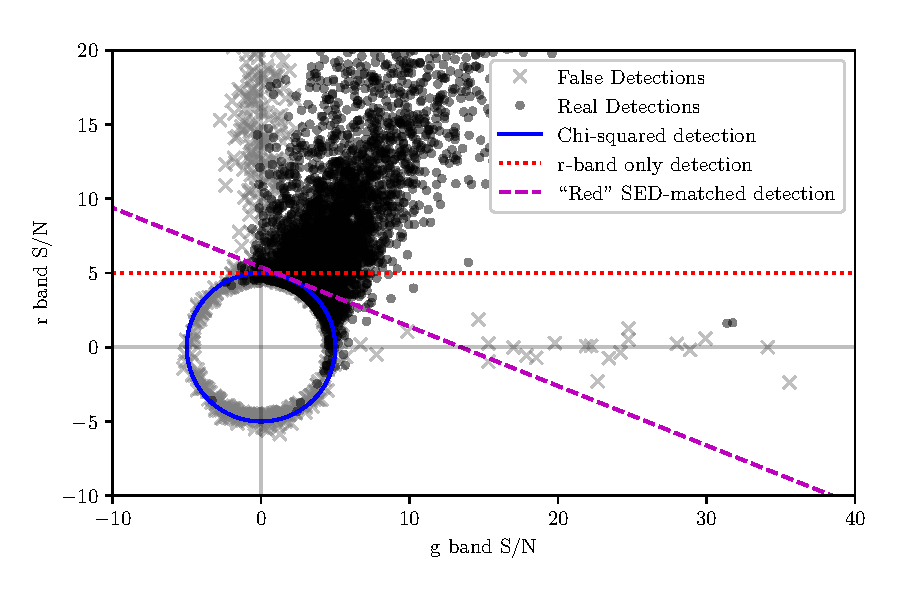
\includegraphics[width=0.8\textwidth]{sed-matched}
    \caption{SED-matched and ``chi-squared'' detection filters.  The
      faint points are (chi-squared) peaks above $3 \sigma$ detected
      in a set of 16 images in each of $g$ and $r$ bands taken with
      the Dark Energy Camera.  The dense set of points near zero are
      primarily due to noise.  The main locus of points correspond to
      real stars and galaxies with typical colors.  The points
      clustered around the horizontal axis are primarily artifacts
      such as cosmic rays affecting one of the $g$-band images.  The
      points clustered around the vertical axis include $r$-band
      artifacts as well as intrinsically red sources.  In theory, the
      sources due to noise should be distributed symmetrically; in
      practice, sky-estimation biases tend to leave the bands
      correlated.  The Chi-squared detection method selects as sources
      all sources outside the circle (including, in the naive
      formulation, sources with negative flux in both bands).  A
      single-band detection filter selects all sources above a
      vertical or horizontal detection threshold.  Our ``red''
      SED-matched filter selects sources where the fluxes in the two
      bands are consistent with a red SED (in this case, a $g - r$
      color of 1).  Note that the threshold line is roughly orthogonal
      to the line between the false positives and the true positives;
      it separated them efficiently.
      \label{fig:sedmatched}
    }
  \end{center}
\end{figure}



\subsection{Comments}

\paragraph{Chi-squared coadd} And how it is different than this.

\paragraph{You always have a prior} And if you don't think you have a prior,
you're probably using a dumb prior.

\paragraph{How much does it hurt if the SED is wrong?} (It's just like having a wrong PSF model.)


\section{Experiments}

\subsection{Sloan Digital Sky Survey}

Here we present some proof-of-concept experiments on Sloan Digital Sky
Survey (SDSS) data from the Stripe 82 region \cite{sdss}.

% FIXME -- The results show XYZ...

\paragraph{Input data selection.}
We select input exposures to include as follows.  Using the
``window\_flist'' table for SDSS Data Release 9 \cite{dr9}, we select
photometric exposures from camera column 3, with RA in the range
$[45.15, 45.85]$ and Dec in the range $[-0.2, -0.1]$.  This results in
$109$ fields from $23$ unique runs, which are listed in
\tabref{tab:fields}.

\paragraph{\Detmap\ and resampling.}
For each input image, we take the PSF to be the double-Gaussian model
computed by the SDSS \emph{Photo} pipeline \cite{photo}, and compute
the \detmap.  Since SDSS DR9 images are already in sky-subtracted,
calibrated ``nano-maggies'', we do not need to apply a calibration
factor to convert them to common units, nor do we need to remove a sky
background level.  We set to zero any image pixels that are masked as
saturated, interpolated, cosmic ray, ghost, or ``not checked'' (close
to the image boundaries).
% 'INTERP', 'SATUR', 'NOTCHECKED', 'GHOST', 'CR'
We compute the per-pixel noise ($\sigma_1$) based on a Gaussian
approximation of the Poisson errors from the mean sky level, plus dark
current and read noise, as recommended by the SDSS
team.\footnote{\niceurl{http://data.sdss3.org/datamodel/files/BOSS\_PHOTOOBJ/frames/RERUN/RUN/CAMCOL/frame.html}}


For each of the $u$, $g$, $r$, $i$ and $z$ bandpass filters
(``bands''), we resample to a common pixel grid and then compute a
per-band \detmap\ as per \eqnref{eq:onebandmap}.  The common pixel
grid is defined by a WCS tangent-plane projection centered on our
patch of interest with the nominal SDSS pixel scale (0.396 arcseconds
per pixel) and image size $4096 \times 2048$ \cite{wcs}.  Since the
SDSS pipeline adds a 128-pixel overlap between neighboring fields in a
run, we first build a \detmap\ for each run, averaging values in the
overlapping regions to avoid double-counting, then combine these
per-run \detmap s as per \eqnref{eq:onebandmap}.  For resampling we
use a third-order Lanczos kernel.

% We track the inverse-variance on a per-pixel basis

\paragraph{Background correction.}
We find that there is considerable spatially-coherent structure in our
combined \detmap s, which we suspect is due to slightly biased
background subtraction in the SDSS pipeline code.  We estimate and
remove a residual background as follows.  After masking all pixels
above 5 sigma, we compute the median value within each cell of a $\sim
100 \times 100$-pixel grid, and interpolate between these values with
a third-order B-spline.  The resulting background-subtracted \detmap s
have no apparent background structure (by eye) and their pixel
distributions are closer to Gaussian.  See \figref{fig:bg}.

\paragraph{Detection}
In this \doctype\ we are not concerning ourselves with blended
objects, so we identify peaks in the \detmap\ naively.  We find
pixels above the desired threshold, expand by a 2-pixel radius, and
find the connected components.  For each component, we return the peak
pixel, ignoring other peaks within the component.


We construct a series of spectral energy distributions (SEDs),
building the combined \detmap\ and running the peak detection
algorithm for each.  A standard approach for detecting objects in
imaging from multiple bands is to weight each band by its
signal-to-noise.  This is equivalent to assuming a flat spectrum, or
zero color.  Our SED-matched filters weight each band according to
both the amount of flux we expect to see in the band, and its
signal-to-noise.  The SEDs we use here include ``Flat'' (expected
color $g = r = i$), ``Red'' ($g-r = r-i = 1$), ``Blue'' ($g-r = r-i =
-1$), and four points lying approximately along the stellar locus
($(g-r, r-i)$ colors $(0.5,0.2)$, $(1.0,0.4)$, $(1.4,0.7)$, and
$(1.4,1.4)$.  In the experiments here we will compare the detection
strengths in the different SEDs.  In practice we would return the
union of peaks detected in this way.



% XXX: Verify this statement
% XXX: Cite ``standard approach''
% XXX: Advice on what to do in practice?

\paragraph{Results}
In \figref{fig:redblue} we show that objects with red colors in the
SDSS catalog are detected more strongly by our SED-matched Red filter
than a Flat SED (which corresponds to the traditional multi-band
detection approach).  There are very few objects that the Blue
SED-matched filter detects more strongly than the Flat or Red filters;
astrophysical objects with blue colors (bluer than 0 in the AB system)
are rare.

% (in the AB system of SDSS)

In \figref{fig:colorcolor} we show, in color-color space, the sources
detected by each of our SED-matched filters.  As expected, each filter
is most sensitive to sources in a given region of color-color space.

% FIXME -- show strongest detections for each SED.

In \figref{fig:missed} we show postage-stamp images of sources that
are detected by our SED-matched filters and not detected by a
traditional approach.  In \figref{fig:added} we show in color-color
space the additional objects that are detected as we apply a sequence
of SED-matched filters.



\subsection{Simulations}

---Single exposure, single band

---Multiple exposures (different PSFs, sky), single band

---Multiple exposures, multiple bands









\begin{table}
\begin{center}
\begin{tabular}{|r|r|r|}
\hline
Run & Min field & Max field \\
\hline
1752 & 163 & 166 \\
1887 & 107 & 111 \\
2578 & 112 & 116 \\
2589 & 200 & 204 \\
2700 & 168 & 171 \\
2738 & 220 & 224 \\
2820 & 168 & 172 \\
2861 & 86 & 90 \\
2873 & 211 & 215 \\
3362 & 169 & 173 \\
3384 & 671 & 675 \\
3461 & 20 & 24 \\
4128 & 425 & 429 \\
4157 & 178 & 181 \\
4198 & 664 & 668 \\
4207 & 673 & 677 \\
4849 & 757 & 760 \\
4858 & 656 & 660 \\
4874 & 723 & 727 \\
4905 & 304 & 307 \\
4927 & 654 & 658 \\
4933 & 665 & 668 \\
4948 & 245 & 249 \\
\hline
\end{tabular}
\caption{SDSS fields included in the experiments.  All fields are from
  camera column (``camcol'') 3.  The minimum and maximum (inclusive)
  fields are listed.\label{tab:fields}}
\end{center}
\end{table}



\begin{figure}
\begin{center}
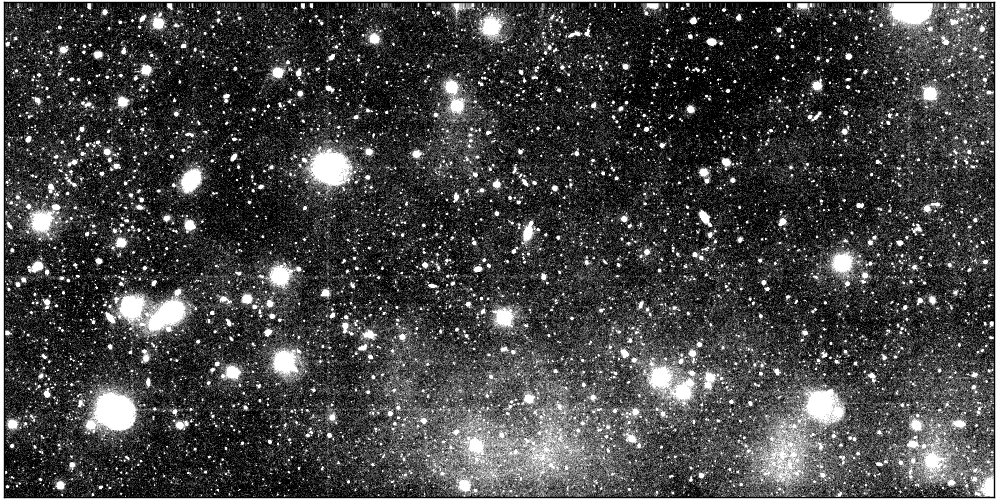
\includegraphics[width=0.7\textwidth]{detect-r-00} \\
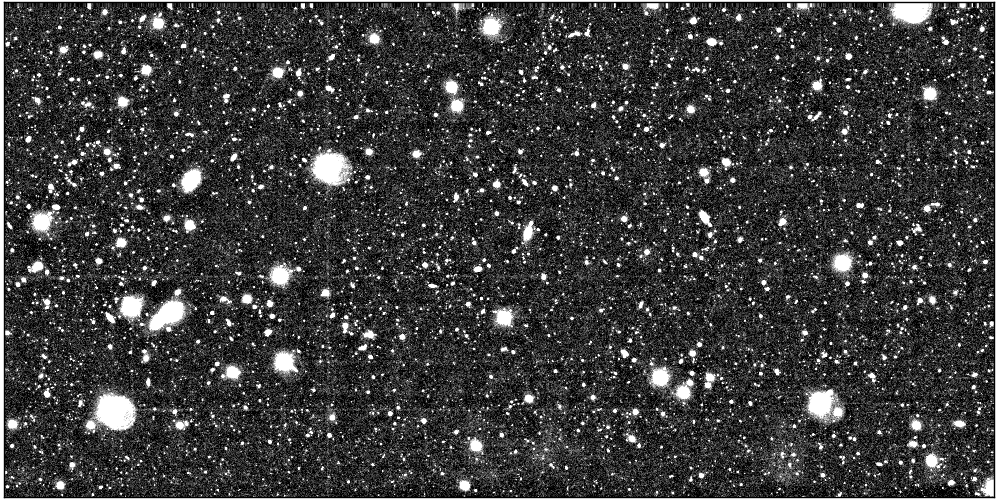
\includegraphics[width=0.7\textwidth]{detect-r-01} \\
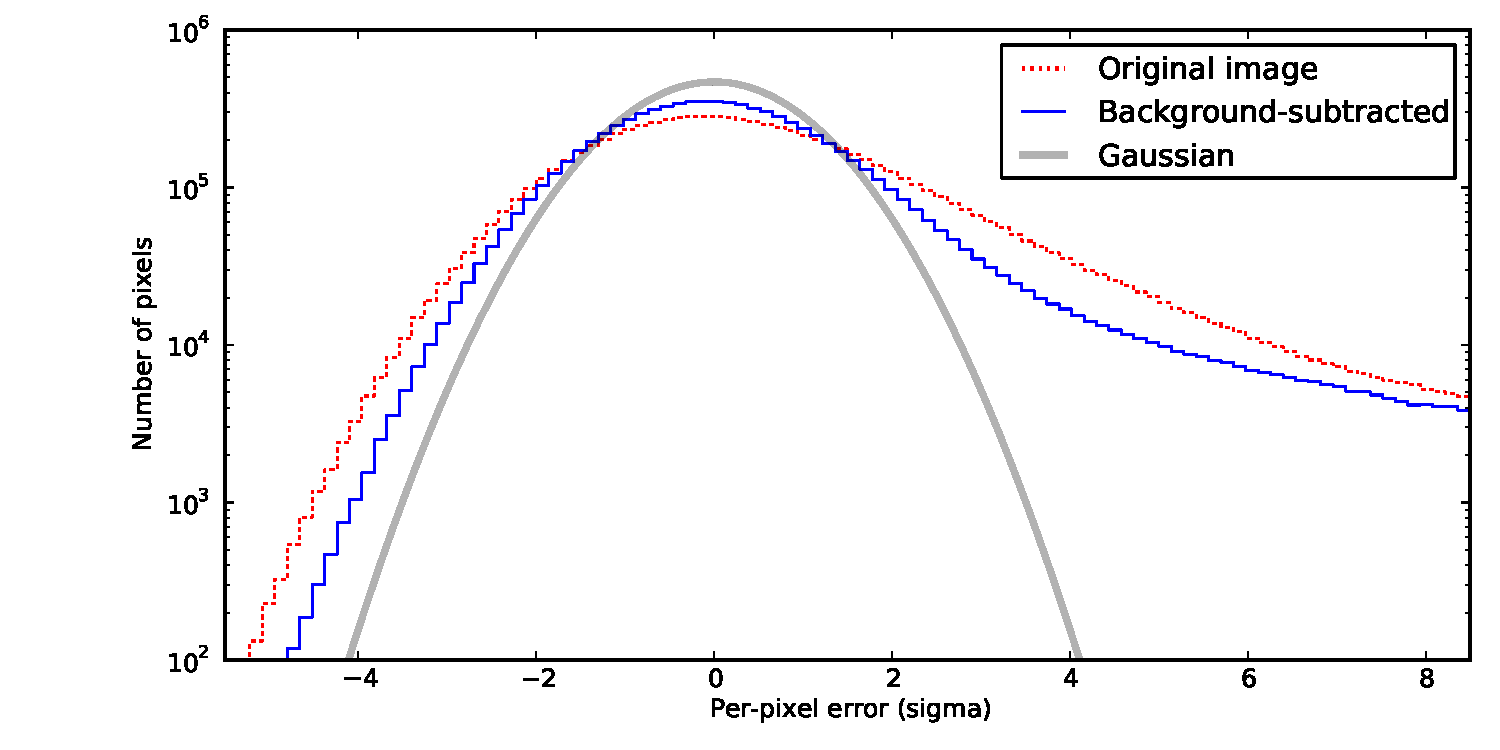
\includegraphics[width=0.8\textwidth]{detect-r-02}
\caption{Residual background subtraction.  \textbf{Top:} combined
  \detmap\ for the SDSS $r$ band, combining images from 23 runs.
  There are clear patterns in the background level.  \textbf{Middle:}
  after estimating and removing the residual background as described
  in the text, the background appears more flat.  \textbf{Bottom:}
  after removing the background, the pixel error statistics are closer
  to Gaussian, though the distribution is still significantly
  broader than expected.\label{fig:bg}}
\end{center}
\end{figure}


\begin{figure}
\begin{center}
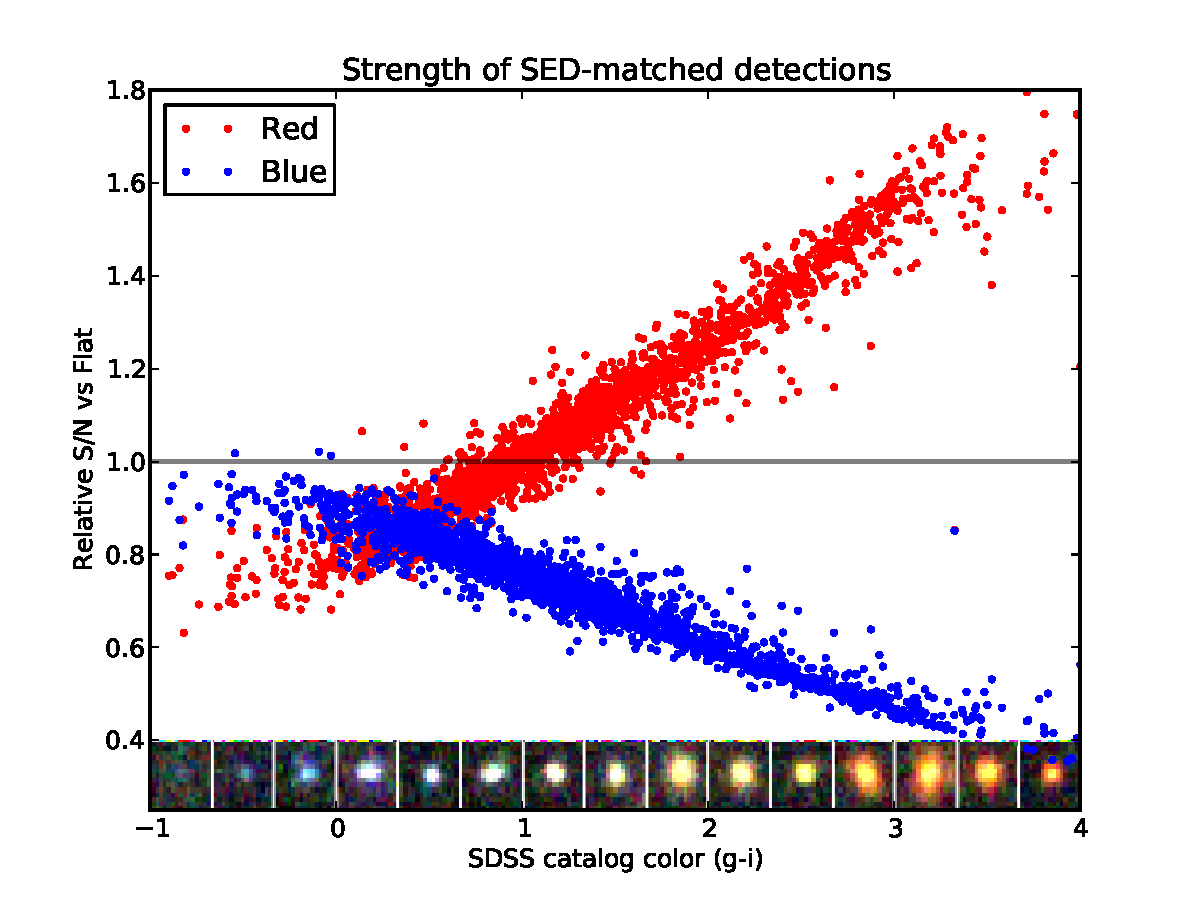
\includegraphics[width=0.8\textwidth]{mdetect-11}
\caption{Detection strengths in the Red, Flat, and Blue SED-matched
  filters, versus SDSS-measured colors.  We performed a spatial match
  between our detected sources and SDSS sources (from the DR7 CasJobs
  database ``Stripe82''; \cite{annis}) within 1 pixel.  Redder objects
  in $g-i$ are detected more strongly in the Red SED-matched filter
  than Flat or Blue.  The handful of objects with significantly blue
  colors are detected more strongly with the Blue filter.
  \label{fig:redblue}}
\end{center}
\end{figure}


\begin{figure}
\begin{center}
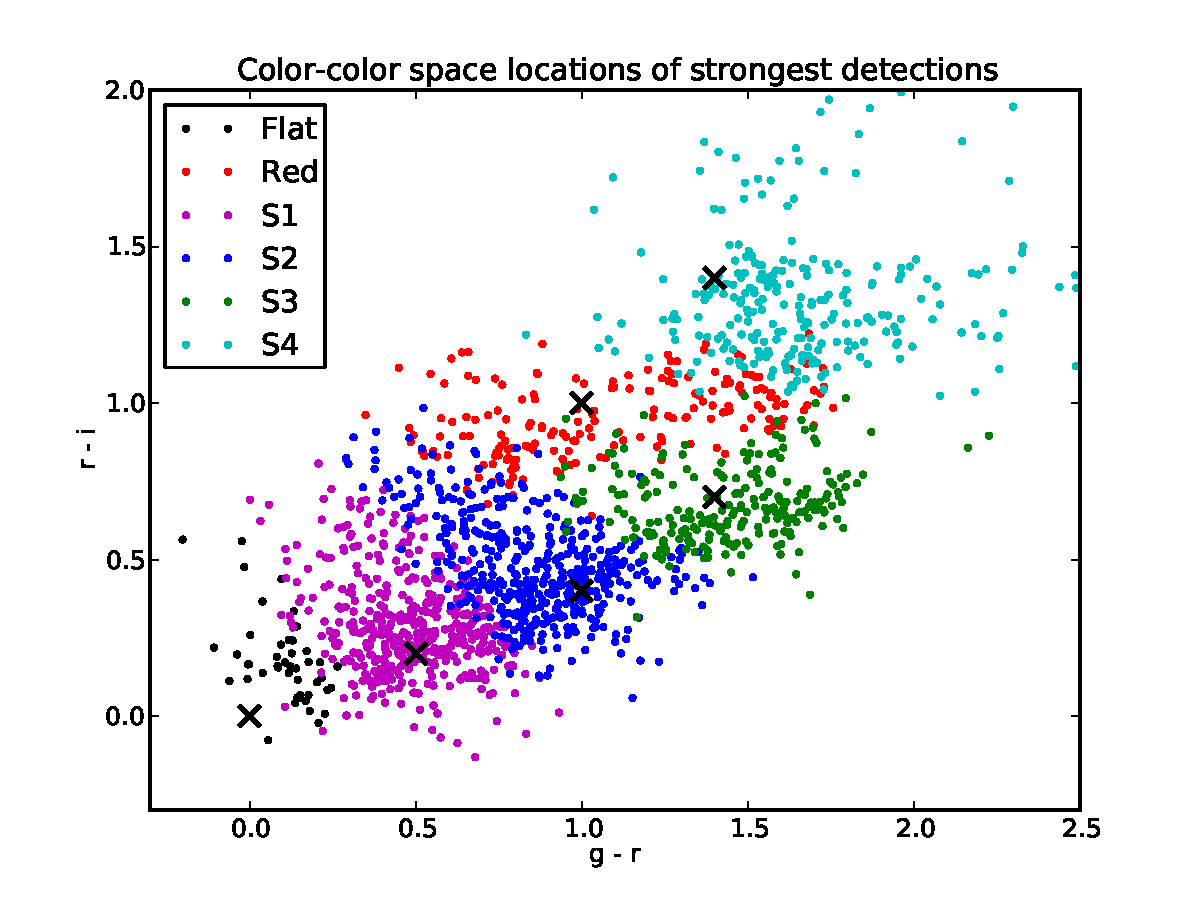
\includegraphics[width=0.8\textwidth]{mdetect-17}
\caption{Color-color space locations of sources detected most strongly
  by each of the filters.
  The color measurements are from the SDSS
  Stripe82 coadd catalog \cite{annis}, matched to
  our detections using a 1-pixel matching radius.
  It is clear that
  our different SED-matched filters are tuned to detect objects in
  particular regions of color-color space.  The ``X'' marks indicate
  the color each SED-matched filter is tuned for.  Note that many of
  the sources are detected above a given detection threshold by
  several of the SED-matched filters; here each source is assigned to
  the filter by which it is detected most strongly.
  \label{fig:colorcolor}}
\end{center}
\end{figure}


\begin{figure}
\begin{center}
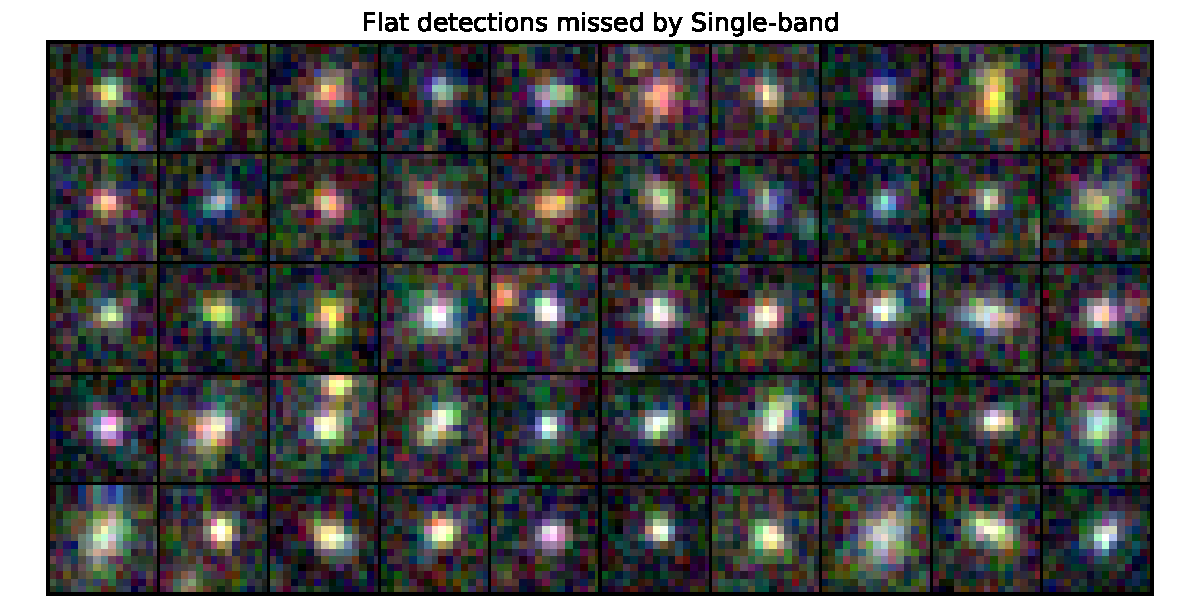
\includegraphics[width=0.8\textwidth]{mdetect-14}
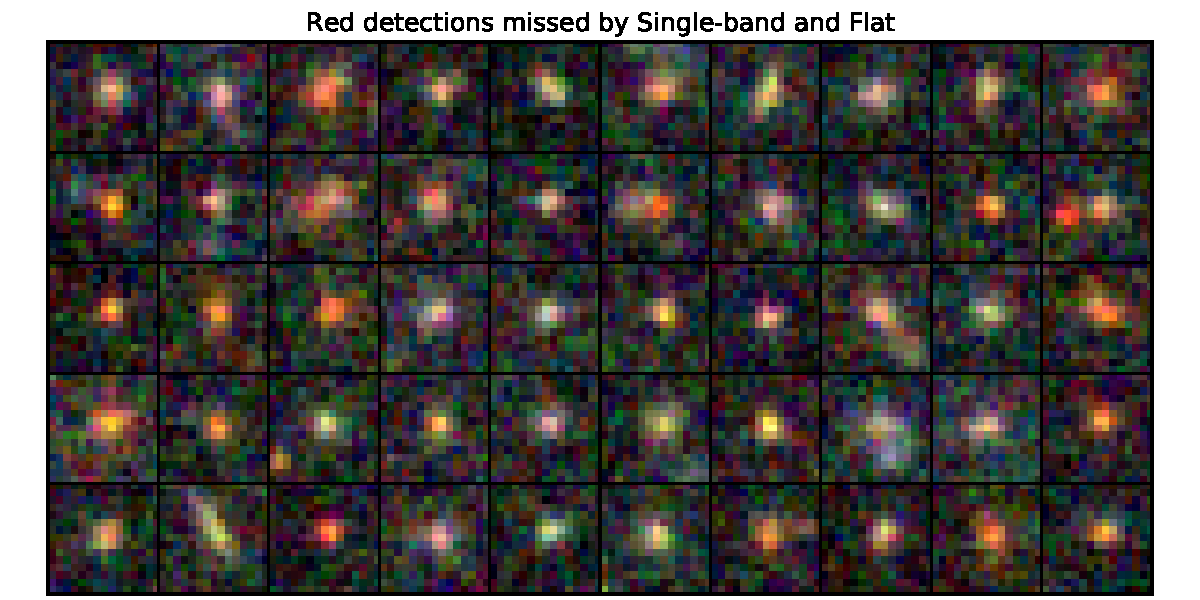
\includegraphics[width=0.8\textwidth]{mdetect-15}
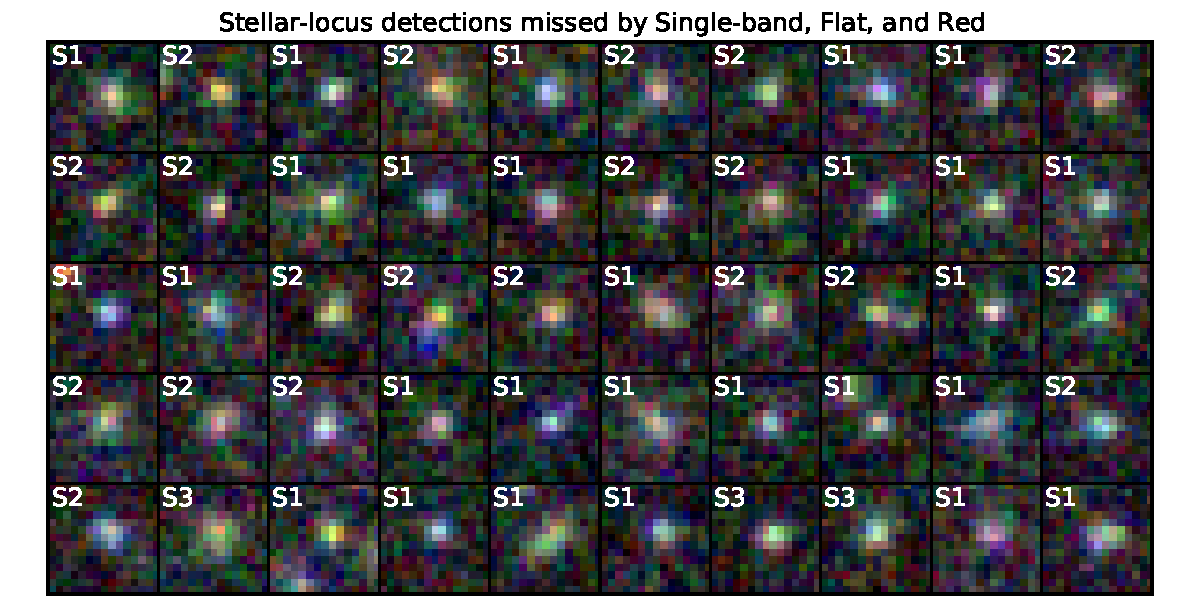
\includegraphics[width=0.8\textwidth]{mdetect-16}
\caption{Sources detected by our SED-matched filters and not by a
  ``traditional'' approach; full caption on next page\label{fig:missed}}
\end{center}
\end{figure}

\addtocounter{figure}{-1}
\begin{figure}
\begin{center}
\caption{[figure previous page] Sources detected by applying a
  sequence of SED-matched filters.  We start with sources detected by
  a ``traditional'' approach that takes the union of single-band
  detections in each of the $g$, $r$, and $i$ filters.  We then apply,
  in sequence, our Flat, Red, and Stellar locus SED-matched filters.
  Each panel shows the sources detected by the new filter and not
  detected by previous filters, in order of decreasing
  signal-to-noise.  In order to make the objects easier to see, we
  have increased the detection threshold to $20 \sigma$.}
\end{center}
\end{figure}

\begin{figure}
\begin{center}
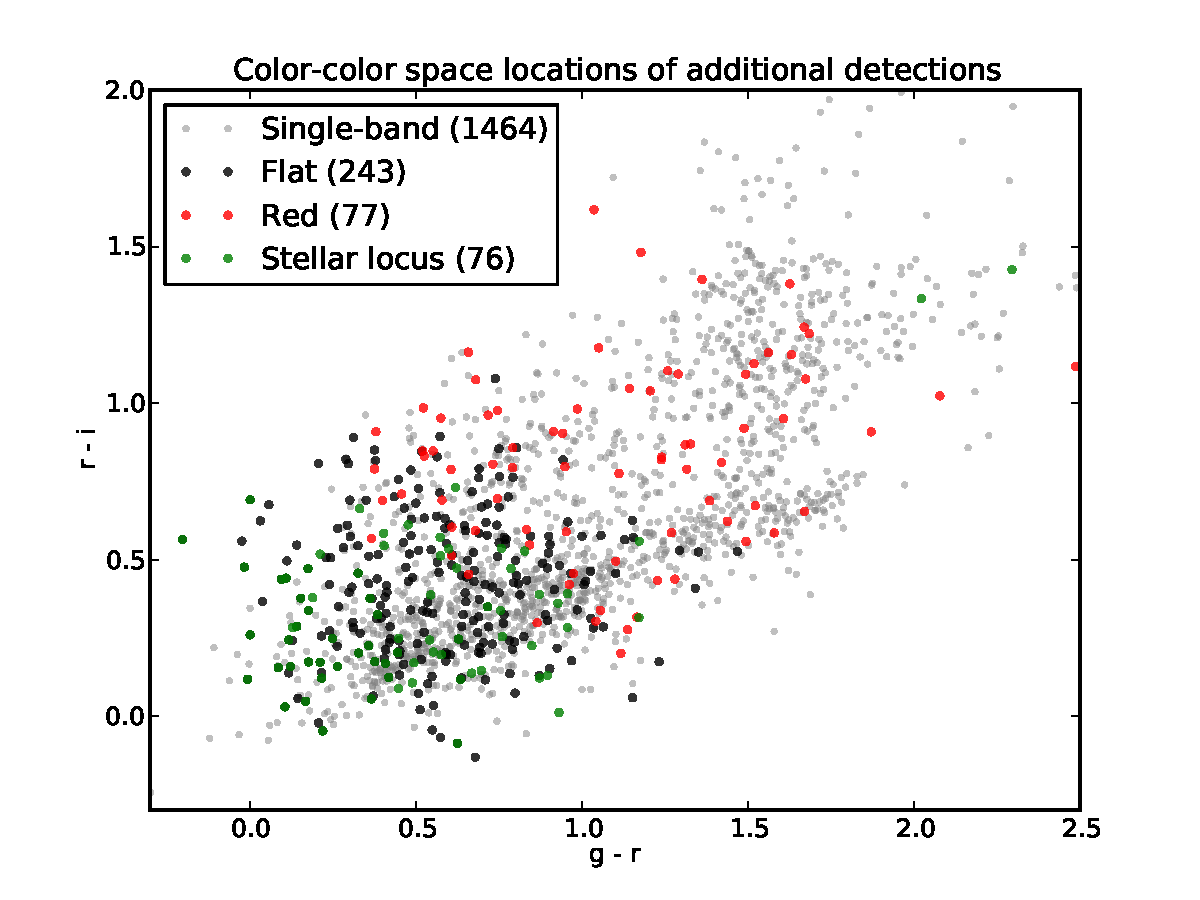
\includegraphics[width=0.8\textwidth]{mdetect-18}
\caption{Color-color space locations of additional sources detected as
  additional SED-matched filters are applied.  We start by taking all
  single-band detections in the $g$, $r$, and $i$-band filters.  Next,
  we add sources detected by the Flat SED-matched filter, then the Red
  filter, then a set of filters along the stellar locus.  Each
  subsequent SED-matched filter detects sources that are missed (at a
  fixed detection threshold) by the previous filters.
  %The color measurements are from the SDSS
  %Stripe82 coadd catalog \cite{annis}, matched to
  %our detections using a 1-pixel matching radius.
  \label{fig:added}}
\end{center}
\end{figure}


\section{Discussion}

--similarities and differences from Szalay et al 19999 -- SED-matched
filters $\sim$ ``optimal subspace filtering''

--galaxy detection?

--No weights go to zero -- all images contribute *something*, in
proportion to t he information they bring.  Contrast with lucky
imaging and some co-adding schemes.

--sub-pixel shifts: lower threshold so that max pixel is above
threshold; post-process to cut out peaks that really were below
threshold.


\section{Conclusions}

[[What to do with a detection image; how to proceed.  Build models,
    fit simultaneously to all images in the ``stack''.]]

[[Practicalities: bad pixels / masks, interpolation, etc]]

\acknowledgements

Ben Weiner (University of Arizona),
Julianne Dalcanton (University of Washington),
Brad Holden (UCO/Lick Observatories),
Micha Gorelick (Fast Forward Labs),
Robert Lupton, Steve Bickerton, Paul Price, and Craig Loomis (Princeton)


%\bibliographystyle{plain}
%\bibliography{coadd}



\appendix

\section{Appendices}

\subsection{Optimal linear detection}
\label{app:lindet}

Let us assume that there exists a linear filter whose output allows
optimal detection of isolated point sources.  That is, we seek a
(two-dimensional) set of coefficients $a_{\ivec}$ that, when
correlated with the image $I_{\jvec}$, produces a map $M_{\jvec}$
whose peak is the likely location of the point source.  See
\figref{fig:detmap}.


The linear filtering (correlation) operation is
\begin{equation}
M_{\jvec} = \sum_{\iina} a_{\ivec} \, I_{\ivec + \jvec}
\label{eq:detmap1}
\end{equation}
where $\mathcal{A}$ is the support of $\avec$ (integer pixel
positions), and the center of $\avec$ is $\coord{0}{0}$.  We will
demand that the elements of $\avec$ are non-negative and sum to unity.

Inserting \eqnref{eq:modelimg}, we get
\begin{eqnarray}
M_{\jvec} &\drawnfrom& \sum_{\iina}
  I_k \, a_{\ivec} \, \psfat{\ivec + \jvec - \kvec} + \gaussx{0}{\sigma_1^2}
  \\
&\drawnfrom& \gaussx{ I_k \sum_{\iina} a_{\ivec} \, \psfat{\ivec + \jvec - \kvec}}%
    {\sum_{\iina} a_{\ivec}^2 \, \sigma_1^2}
\end{eqnarray}
and the per-pixel signal-to-noise in the map is
\begin{equation}
%  \signoise_{D_{\jvec}} = \frac{I_k \, \sum_{\iina} a_{\ivec} \, \psfat(\ivec + \jvec - \kvec)}{\sigma_1 \sqrt{\sum_{\iina} a_{\ivec}^2}}
  \snr{M_{\jvec}} = \frac{I_k \, \sum a_{\ivec} \, \psfat{\ivec + \jvec - \kvec}}{\sigma_1 \sqrt{\sum_{\ivec} a_{\ivec}^2}} \quad .
  \label{eq:detmapsn1}
\end{equation}

We want to choose coefficients $a_{\ivec}$ to maximize the 
signal-to-noise at the true pixel position of the source,
$\kvec$.  Rewriting the expression using dot-products and
norms\footnote{All norms in this \doctype\ are $\ell_2$ norms: $\norm{X} =
  \sqrt{\sum_i X_i^2}$.}, treating the two-dimensional images
$a_{\ivec}$ and $\psfat{\ivec + \jvec - \kvec}$ as vectors indexed by
$\ivec$, we have:
\begin{eqnarray}
  %\signoise_{D_{\jvec}} &=& \frac{I_k \, \avec \cdot \bm{\psfat(\jvec-\kvec)}}{\sigma_1 \sqrt{\avec \cdot \avec}} \\
  \snr{M_{\jvec}} &=& \frac{I_k \, \avec \cdot \bm{\psfat{j-k}}}{\sigma_1 \sqrt{\avec \cdot \avec}} \label{eqn:psfdotprod} \\
 &=& \frac{I_k \, \norm{\avec} \norm{\bm{\psfat{j-k}}} \cos \theta}{\sigma_1 \norm{\avec}} \\
 &=& \frac{I_k \, \norm{\bm{\psfat{j-k}}} \cos \theta}{\sigma_1}
\end{eqnarray}
where $\theta$ is a generalized angle between $\avec$ and $\bm{\psfat{j-k}}$.
At the pixel position of the source, $\kvec$,
\begin{equation}
\snr{M_{\kvec}} = \frac{I_k \, \norm{\bm{\psfat{0}}} \cos \theta}{\sigma_1}
\label{eqn:sndsingle}
\end{equation}
Clearly this is maximized when $\theta = 0$, \ie, when $\avec$ is a
multiple of $\bm{\psfat{0}}$, the PSF evaluated at a grid of integer
pixel positions.  Since we have defined both the PSF and coefficients
$a$ to sum to unity, we find that the optimal linear filter for
detection is given by:
\begin{equation}
%  a_{\ivec} = \psfat{\ivec} \quad ,
\avec = \bm{\psfat{0}} \quad ,
\end{equation}
which means that the operation of \emph{correlating} the image with
its PSF produces a map with optimal signal-to-noise.  Repeating
equation \ref{eq:detmap1}, we have found that the map $M_{\jvec}$ can
be computed by correlating the image with its PSF:
\begin{equation}
M_{\jvec} = \sum_{\iina} \psfat{\ivec} \, I_{\ivec + \jvec} \quad ,
\end{equation}
where, as before, $\mathcal{A}$ is the support of the PSF.
% and
%$\psfat{\ivec} = \psfat{\ivec}$ is an image of the PSF evaluated at
%integer pixel positions $\ivec$.

The signal-to-noise in this map at the true source pixel
position $\kvec$ is
\begin{equation}
\snr{M_{\kvec}} = \frac{I_k \, \norm{\bm{\psfat{}}}}{\sigma_1} \quad .
\end{equation}


\subsubsection{Optimality}
\label{sec:optsingle}

We compute the variance of the detection map estimator
(\eqnref{eq:detmap}), and show that is equal to the Cram\'er--Rao
bound.  Substituting our image model into the detection map,
\begin{eqnarray}
D_{\jvec} &=& \frac{1}{\psfnorm^2} \sum_{i} \psfat{\ivec} \,
I_{\ivec + \jvec}
\\
& \drawnfrom & \frac{1}{\psfnorm^2} \sum_{i} \psfat{\ivec} \,
\gaussx{F \, \psfat{\ivec + \jvec - \kvec}}{\sigma_1^2}
\end{eqnarray}
and at the true source position, $\jvec = \kvec$;
\begin{eqnarray}
%D_{\jvec} &\drawnfrom& 
%\frac{1}{\psfnorm^2} \sum_{i}
%\gaussx{F \, \psfat{\ivec}^2}{\psfat{\ivec}^2 \sigma_1^2}
%
D_{\kvec} &\drawnfrom& \frac{1}{\psfnorm^2} \gaussx%
{F \, \sum_{i} \psfat{\ivec}^2}%
{\sum_{i} \psfat{\ivec}^2 \sigma_1^2}
\\
D_{\kvec} &\drawnfrom& \gaussx%
{F}{\frac{\sigma_1^2}{\psfnorm^2}}
\end{eqnarray}
so the variance of the estimator is $\var{D} = \frac{\sigma_1^2}{\psfnorm^2}$.

Meanwhile, the Fisher Information for $F$ given pixel values $I_{\jvec}$ is
\begin{eqnarray}
  I(F) &=& -\mathbb{E}_{I_{\jvec}} \left[ \frac{\partial^2 \log P(\{ I_{\jvec} \} | F)}{\partial F^2} \right]
\end{eqnarray}
and with pixel values $I_{\jvec}$ the likelihood is
\begin{eqnarray}
  I_{\jvec} &\drawnfrom& \gaussx{F \psf_{\jvec}}{\sigma_1^2} \\
  P(\{ I_{\jvec} \} | F) &=& \prod_{\jvec} \frac{1}{\sqrt{2 \pi \sigma_1^2}} \exp \left( -\frac{(I_{\jvec} - F \psf_{\jvec})^2}{2 \sigma_1^2} \right) \\
  %\log P(\{ I_{\jvec} \} | F) &=& \sum_{\jvec} \log \frac{1}{\sqrt{2 \pi \sigma_1^2}} + \sum_{\jvec} -\frac{(I_{\jvec} - F \psf_{\jvec})^2}{2 \sigma_1^2} \\
  %\frac{\partial}{\partial F} \log P(\{ I_{\jvec} \} | F) &=& \sum_{\jvec} \frac{(I_{\jvec} - F \psf_{\jvec}) \psf_{\jvec}}{\sigma_1^2} \\
  \frac{\partial^2}{\partial F^2} \log P(\{ I_{\jvec} \} | F) &=& \sum_{\jvec} -\frac{\psf_{\jvec}^2}{\sigma_1^2}
\end{eqnarray}
which is independent of $I_{\jvec}$, so
\begin{eqnarray}
  I(F) &=& \frac{\norm{\psf}^2}{\sigma_1^2}
\end{eqnarray}
from which we see that the estimator $D$ saturates the Cram\'er--Rao bound.

\subsubsection{Norm of a Gaussian PSF}
\label{app:gaussnorm}
For a Gaussian PSF with standard deviation $\psfw$ pixels,
\begin{eqnarray}\displaystyle
\psf^G(x,y) &=& \frac{1}{2 \pi \psfw^2} \exp{\left(-\frac{x^2}{2 \psfw^2}\right)} \exp{\left(-\frac{y^2}{2 \psfw^2}\right)}
\end{eqnarray}
the norm is% approximately:
\begin{eqnarray}
\norm{\bm{\psf^G}} &=& \sqrt{ \sum_{x} \sum_{y} \left(\frac{1}{2 \pi \psfw^2} \exp{\left(-\frac{x^2}{2 \psfw^2}\right)} \exp{\left(-\frac{y^2}{2 \psfw^2}\right)} \right)^2} \\
%\left(\norm{\psf^G}\right)^2 &\simeq& \iint \frac{1}{4 \pi^2 \psfw^4} \exp{\left(-\frac{x^2}{\psfw^2}\right)} \exp{\left(-\frac{y^2}{\psfw^2}\right)} \mathrm{d}x \, \mathrm{d}y \\
\norm{\bm{\psf^G}} &\simeq& \sqrt{\iint \frac{1}{4 \pi^2 \psfw^4} \exp{\left(-\frac{x^2}{\psfw^2}\right)} \exp{\left(-\frac{y^2}{\psfw^2}\right)} \mathrm{d}x \, \mathrm{d}y} \\
\norm{\bm{\psf^G}} &\simeq& \frac{1}{2 \sqrt{\pi} \psfw}
\end{eqnarray}
so the \detmap\ has signal-to-noise at the true source position $\kvec$,
\begin{equation}
\snr{D_{\kvec}^G} = \frac{I_k}{2 \sqrt{\pi} \psfw \sigma_1 } \quad .
\label{eqn:sndsinglegauss}
\end{equation}

Note, however, that we have defined the point-spread function
$\psfat(\cdot)$ to be the \emph{pixel-convolved} response, so it cannot
be exactly Gaussian if the pixel response is assumed to be a boxcar
function.  In practice, however, a two-dimensional Gaussian with
variance $v^2$ correlated with a two-dimensional boxcar function is
well approximated by a Gaussian with variance $v^2 + \frac{1}{12}$, as
long as $v \gtrsim \frac{1}{2}$.

% figure showing this?




\subsubsection{Why not signal-to-noise-squared?}
In correlating the image with the PSF, it looks like the
\detmap\ weights pixels by their signal-to-noise, rather than
signal-to-noise \emph{squared}.  This apparent conflict can be
resolved by scaling the pixel values so that each pixel is an estimate
of the same quantity.  That is, we want to estimate the total source
counts $F$, but the pixels contain estimates of the source counts
scaled by the PSF, $F \psf$; we must undo this scaling by multiplying
the pixels by $1/\psf$.

Given a source at position $\kvec$, we define the image $K$ whose
pixels each contain an estimate of the total source counts:
\begin{eqnarray}
  K_{\jvec} &=& \frac{1}{\psfat{\jvec-\kvec}} S_{\jvec}  \\
  K_{\jvec} &\drawnfrom& \frac{1}{\psfat{\jvec-\kvec}} \, \gaussian{I_k \, \psfat{\jvec-\kvec}\, , \, \sigma_1^2} \\
  K_{\jvec} &\drawnfrom& \gaussian{I_k \, , \, \frac{\sigma_1^2}{\psfat{\jvec-\kvec}^2}} \quad .
\end{eqnarray}

The signal-to-noise remains the same, since we have just scaled the
values:
\begin{eqnarray}
\snr{K_{\jvec}} &=& \frac{I_k \, \psfat{\jvec-\kvec}}{\sigma_1} \\
\snr{K_{\jvec}} &=& \snr{S_{\jvec}} \quad .
\end{eqnarray}


As before, the \detmap\ pixels are a linear combination of the
(shifted) pixels of the $K$ image with weights $b_{\ivec}$:
\begin{eqnarray}
D_{\jvec}^\star &=& \sum_{\ivec} b_{\ivec} \, K_{\ivec+\jvec} \\
&\drawnfrom& \sum_{\ivec} b_{\ivec} \, \gaussian{I_k \,,\, \frac{\sigma_1^2}{\psfat{\ivec+\jvec-\kvec}^2}} \\
&\drawnfrom& \gaussian{I_k \sum_{\ivec} b_{\ivec} \,,\, \sum_{\ivec} \frac{b_{\ivec}^2 \sigma_1^2}{\psfat{\ivec+\jvec-\kvec}^2}}
\end{eqnarray}
and the signal-to-noise in that \detmap\ at pixel $\kvec$ is
\begin{eqnarray}
\snr{D_{\kvec}^\star} &=& \frac{I_k \sum_{\ivec} b_{\ivec}}{\sigma_1 \sqrt{\sum_{\ivec} \frac{b_{\ivec}^2}{\psfat{\ivec}^2}}}
\end{eqnarray}
which is maximized by setting the $b_{\ivec}$
\begin{equation}
b_{\ivec} \propto \psfat{\ivec}^2 \quad :
\end{equation}
proportional to the signal-to-noise \emph{squared}, as expected.

% Derivative is
% d\snr{D_k^\star}/db_k = 
%  \[ \frac{f}{\sigma} [ \frac{1}{\sqrt{\sum_j \frac{b_j^2}{\psfat{j}^2}}}
%                       - \frac{(\sum_j b_j) b_k}{\psfat{j}^2 (\sum_j \frac{b_j^2}{\psfat{j}^2})^{3/2}} ]
% \]
%
% And through some seemingly circular math you get to:
% b_k = \psfat{k}^2 * ( \sum_j (b_j^2 / \psfat(j)^2) ) / (sum_j (b_j))
%
% (you can remove the b_k term from the sums over j if you want, with no effect.)
%
% So b_k = \alpha \psfat{k}^2; substituting that you get:
%
% b_k = \psfat{k}^2 * ( \sum_j ( (\psfat{j}^2 \alpha)^2 / \psfat{j}^2 ) / (sum_j (\psfat{j}^2 \alpha))
%     = \psfat{k}^2 * ( \alpha^2 \sum_j \psfat{j}^2 ) / (\alpha \sum_j(\psfat{j}^2))
%     = \psfat{k}^2 * \alpha



\subsection{Multi-image detection}
\label{app:multidet}

\subsubsection{Optimality}
\label{app:multiopt}
As before, we will show that the estimator $F^{\star}$ in
Equation \ref{eq:onebandmap} saturates the Cram\'er--Rao bound for $F$.

We will consider two images, $A$ and $B$, with PSFs $\psi$ and $\phi$,
respectively, and calibration factors $\kappa_A$ and $\kappa_B$ that
scale image units to flux units.  Per-pixel noise in the two images
will be $\sigma_A$ and $\sigma_B$.  We will assume that the pixel
grids are aligned so that no resampling is necessary.

Given all this, the pixel value for images $A$ and $B$ are drawn from
the distributions
\begin{eqnarray}
  A & \drawnfrom & \gaussx{\frac{F}{\kappa_A} \psi_k}{\sigma_A^2} \\
  B & \drawnfrom & \gaussx{\frac{F}{\kappa_B} \phi_k}{\sigma_B^2}
  \quad .
\end{eqnarray}
The Fisher Information is
\begin{eqnarray}
  I(F) &=& -\mathbb{E}_{A,B} \left[ \frac{\partial^2 \log P(\{ A,B \} | F)}{\partial F^2} \right]
\end{eqnarray}
and assuming that images $A$ and $B$ are statistically independent,
$P(A,B | F) = P(A|F) P(B|F)$.  Following the analysis in
\ref{sec:optsingle}, we find that
\begin{eqnarray}
  I(F) &=& \frac{\norm{\psi}^2}{\kappa_A^2 \sigma_A^2} +
  \frac{\norm{\phi}^2}{\kappa_B^2 \sigma_B^2}
\end{eqnarray}
which equals the variance of the $F^{\star}$ estimator,
$\sigma_{F^{\star}}^2$ as given in Equation \ref{eq:onebandstd}.
Therefore, the estimator saturates the Cram\'er--Rao bound.

\end{document}

